\documentclass[a4paper,12pt]{article}

%%% Работа с русским языком
\usepackage{cmap}					% поиск в PDF
\usepackage{mathtext} 				% русские буквы в фомулах
\usepackage[T2A]{fontenc}			% кодировка
\usepackage[utf8]{inputenc}			% кодировка исходного текста
\usepackage[english,russian]{babel}	% локализация и переносы

%%% Работа с картинками
\usepackage{graphicx}  % Для вставки рисунков
\graphicspath{{images/}{images2/}}  % папки с картинками
\setlength\fboxsep{3pt} % Отступ рамки \fbox{} от рисунка
\setlength\fboxrule{1pt} % Толщина линий рамки \fbox{}
\usepackage{wrapfig} % Обтекание рисунков текстом

%%% Работа с таблицами
\usepackage{array,tabularx,tabulary,booktabs} % Дополнительная работа с таблицами
\usepackage{longtable}  % Длинные таблицы
\usepackage{multirow} % Слияние строк в таблице

%%% Страница

\usepackage{geometry} % Простой способ задавать поля
	\geometry{top=25mm}
	\geometry{bottom=35mm}
	\geometry{left=35mm}
	\geometry{right=20mm}

\author{Мосеевская Валерия, группа 172-3}
\title{\textbf{Flower of Scotland}}

\begin{document} % конец преамбулы, начало документа

\maketitle

\textbf{<<Flower of Scotland>>} (Scottish Gaelic: \textit{Flùr na h-Alba}) is a Scottish song, used frequently at special occasions and sporting events. Although there is no official national anthem of Scotland, <<Flower of Scotland>> is one of a number of songs which fulfil this role, along with the older <<Scots Wha Hae>>, and <<Scotland the Brave>>, amongst others.It was written by Roy Williamson of the folk group the Corries, and presented in 1967, and refers to the victory of the Scots, led by Robert the Bruce, over England's Edward II at the Battle of Bannockburn in 1314.

\tableofcontents

\section{Lyrics}

The song was composed and is sung in English, typically with Scots pronunciation of a few words (e.g. <<Tae>> as opposed to <<To>>). Here is a fine table with the first verse of <<Flower of Scotland>>:

\begin{longtable}{p{5cm}p{5cm}p{5cm}}
    \\
	\textbf{English} & \textbf{Scots} & \textbf{Gaelic} \\
	O Flower of Scotland, & O Flouer o Scotland, & O Fhlùir na h-Alba,\\
	When will we see & Whan will we see & cuin a chì sinn \\
	Your like again, & Yer like again, & an seòrsa laoich \\
	That fought and died for, & That focht an dee'd for, & a sheas gu bàs 'son \\
	Your wee bit Hill and Glen, & Yer wee bit Hill an Glen, & am bileag feòir is fraoich,\\
	And stood against him, & An stuid agin him, & a sheas an aghaidh\\
	Proud Edward's Army, & Prood Edwart's Airmie, & feachd uailleil Iomhair\\
	And sent him homeward, & An sent him hamewart, & 's a ruaig e dhachaidh\\
	To think again. & Tae think again. & air chaochladh smaoin?\\
\end{longtable} 

\section{Popular use}

\subsection{About sport}

The song has been used as a National Anthem by the Scotland national rugby union team, ever since the winger, Billy Steele, encouraged his team-mates to sing it on the victorious Lions tour of South Africa in 1974. The song was adopted as the pre-game anthem during the deciding match of the 1990 Five Nations Championship between Scotland and England, which Scotland won 13–7 to win the Grand Slam. The Scottish Football Association adopted <<Flower of Scotland>> as its pre-game national anthem in 1997 although it was first used by them in 1993. Usually only the first and third verses are sung. At any home International Scotland Rugby union test match the first verse is accompanied by bagpipes followed by the third verse unaccompanied by any instrument.
\begin{wrapfigure}{r}{0.35\linewidth}
	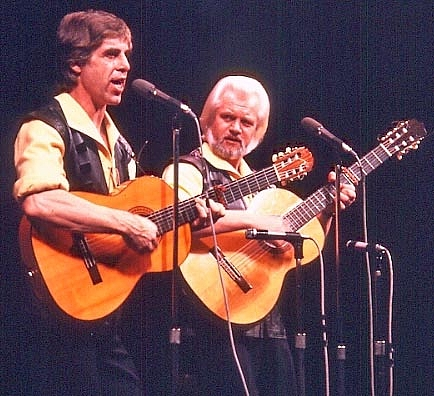
\includegraphics[width=\linewidth]{both}
	\caption{The Corries: Roy Williamson and Ronnie Browne singing}
\end{wrapfigure}

\subsection{About other stuff}

In July 2006, the Royal Scottish National Orchestra conducted an online poll (publicised by Reporting Scotland) in which voters could choose a national anthem from one of five candidates. 10,000 people took part in the poll in which Flower of Scotland came out the winner. The results were as follows:
\vspace{0,5cm}

\begin{tabular}{|p{5cm}|p{2,5cm}|}
    \hline
    \textbf{Tune} & \textbf{Votes (\%)} \\
\hline
	Flower of Scotland & 41\% \\
\hline
	Scotland the Brave & 29\% \\
\hline
	Highland Cathedral & 16\% \\
\hline
	Is There for Honest Poverty & 8\% \\
\hline
	Scots Wha Hae &	6\% \\
\hline
\end{tabular} 
\vspace{0,5cm}
    
Scottish pirate metal band Alestorm have performed a cover of it live and recorded it, which is on their album Captain Morgan's Revenge. In addition, the Canadian Scottish-influenced Celtic Punk band The Real McKenzies have included the song on the album <<Loch'd \& Loaded>> as well a staple in their live performance among many other traditional Scottish ballads.

At the 2012 Summer Olympics opening ceremony, the song was sung at Edinburgh Castle by 53 Scottish children selected from schools across Scotland.

\section{Some lists and illustrations}

\subsection{About panicking}

\begin{itemize}
	\item
	\begin{itemize}
		\item Проблема номер 1.
		\item В статье не нашлось материала для списков разных вариантов, поэтому были предприняты следующие действия: 
		\begin{enumerate}
			\item Немедленная паника
			\item Осознание невозможности отступления за 2 часа до дедлайна
            \item Принятие решения делать дальше
            \item Создание этого списка.
		\end{enumerate}
	\end{itemize}
    \item
	\begin{itemize}
        \item Проблема номер 2.
    		\begin{itemize}
				\item Не нашлось и иллюстраций в статье
				\item К счастью, это поправимо
				\item Поэтому вот фотография автора песни <<Flower of Scotland>> и немного текста про него и его друга, с которым они выступали:
			\end{itemize}
	\end{itemize}
\end{itemize}

\subsection{About Roy Williamson}

%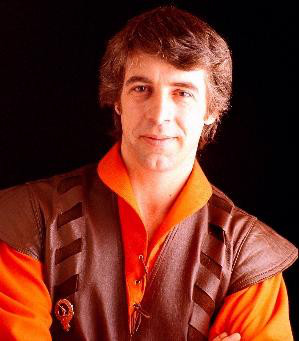
\includegraphics[scale=0.6]{roy1.jpg}
\begin{wrapfigure}{l}{0.3333\linewidth}
	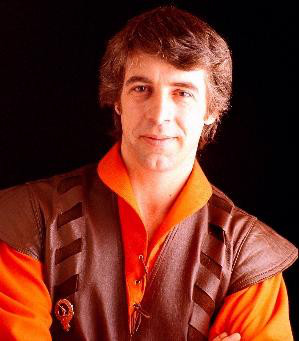
\includegraphics[width=\linewidth]{roy1}
	\caption{Roy Williamson, the author of the song}
\end{wrapfigure} Roy Murdoch Buchanan Williamson (25 June 1936 – 12 August 1990) was a Scottish songwriter and folk musician, most notably with The Corries. Williamson is best known for writing <<Flower of Scotland>>, which has become the de facto national anthem of Scotland used at international sporting events.

\subsection{About Ronnie Browne and <<The Corries>>}

Ronnie Browne (<<The Voice>>) (born Ronald Grant Browne, 20 August 1937 in Edinburgh, Lothian, Scotland), is a Scottish folk musician and founding member of The Corries.

Browne's musical career began when he met Roy Williamson and multi-instrumentalist Bill Smith at Edinburgh College of Art in 1955 and formed the Corrie Folk Trio in 1962. The group was expanded the following year with the addition of female singer Paddie Bell. Shortly after releasing three albums in 1965, Bell left to begin a solo career. With the departure of Smith, the following year, Browne and Williamson continued to perform as a duo now known as The Corries.

%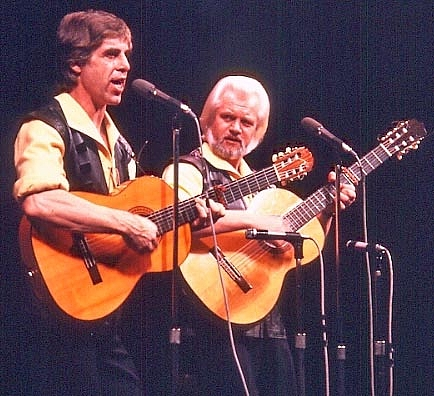
\includegraphics{both.jpg}


\end{document} % конец документа

